\begin{frame}
\frametitle{Системные вызовы}
\begin{itemize}
    \item<1->Системные вызовы - интерфейс между userspace и ядром ОС
    \begin{itemize}
        \item<2->пользовательский код не имеет достаточно привилегий,
             чтобы вызывать код ядра как обычные функции;
        \item<3->системный вызов сопровождается повышением привилегий;
        \item<4->возврат из системного вызова сопровождается понижением
             привилегий.
    \end{itemize}
\end{itemize}
\end{frame}

\begin{frame}
\frametitle{Реализация системных вызовов}
\begin{itemize}
    \item<1->Как реализовать интерфейс системных вызовов?
    \begin{itemize}
        \item<2->способ, как обычно, зависит от архитектуры;
        \item<3->например, в x86 существуют инструкции syscall и sysenter;
        \item<4->но мы посмотрим на другой вариант (более старый).
    \end{itemize}
\end{itemize}
\end{frame}

\begin{frame}
\frametitle{И сново о прерываниях...}
\begin{itemize}
    \item<1->Что происходит, если обработчик прерывания прерывает
         пользовательский код?
    \begin{itemize}
        \item<2->вызывается обработчик прерывания - код ядра;
        \item<3->обработчик прерывания выполняется уже в привилегированном
             режиме.
    \end{itemize}
\end{itemize}
\end{frame}

\begin{frame}
\frametitle{Программные прерывания}
\begin{itemize}
    \item<1->Прерывания можно вызывать программно (и не только сделав ошибку)
    \begin{itemize}
        \item<2->например, в x86 для этого существует специальная инструкция
             int, номер прерывания - параметр инструкции;
        \item<3->выберем запись в IDT и будем использовать ее для системных
             вызовов.
    \end{itemize}
\end{itemize}
\end{frame}

\begin{frame}
\frametitle{Программные прерывания в x86}
\begin{itemize}
    \item<1->С помощью инструкции int в x86 можно генерировать прерывание с
        любым номером
    \begin{itemize}
        \item<2->в том числе и соответствующие исключениям;
        \item<3->в том числе и соответствующие аппаратным прерываниям;
        \item<4->приложения могут натворить бед, если разрешить им
             генерировать прерывания как попало.
    \end{itemize}
\end{itemize}
\end{frame}

\begin{frame}
\frametitle{Дескриптор IDT, поле DPL}
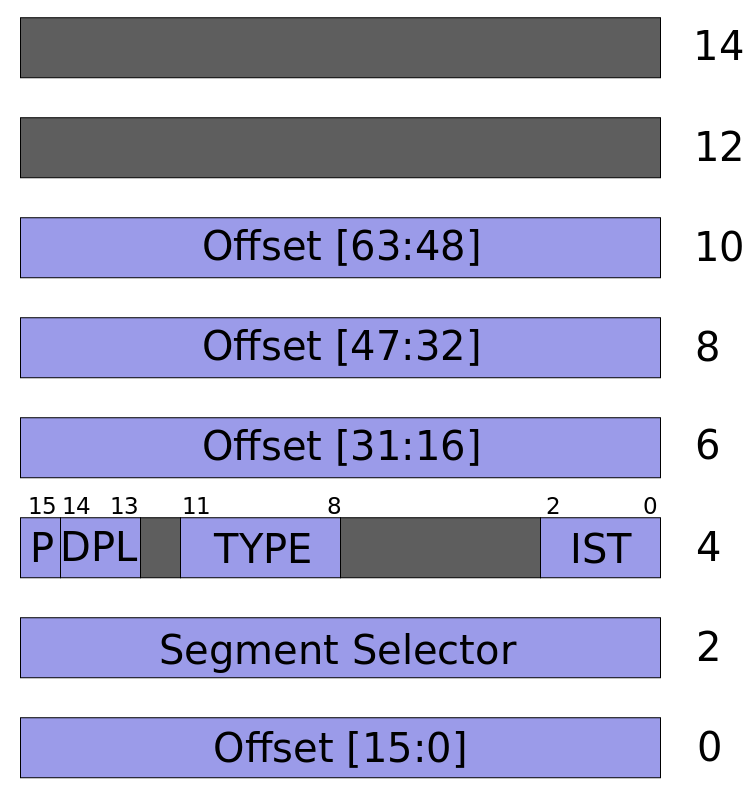
\includegraphics[height=.6\textheight]{desc}
\end{frame}

\begin{frame}
\frametitle{Дескриптор IDT, поле DPL}
\begin{itemize}
    \item<1->DPL дескриптора системного вызова выставляем в 3
    \begin{itemize}
        \item<2->благодаря чему непривилегированный код может генерировать
             это прерывание.
    \end{itemize}
    \item<2->DPL всех остальных дескрипторов выставляем в 0.
\end{itemize}
\end{frame}

\begin{frame}
\frametitle{Стек обработчика прерывания}
\begin{itemize}
    \item<1->При вызове обработчика на стек сохраняются адрес возврата и прочее
    \begin{itemize}
        \item<2->на какой стек все это будет сохранено?
        \item<3->не хочется использовать стек непривилегированного кода
        \begin{itemize}
            \item<4->там может быть не достаточно места;
            \item<5->пользовательский код может делать со своим стеком все
                 что угодно.
        \end{itemize}
    \end{itemize}
\end{itemize}
\end{frame}

\begin{frame}
\frametitle{Отдельный стек для ядра}
\begin{itemize}
    \item<1->Мы хотим использовать отдельный стек для ядра и отдельный
         для userspace
    \begin{itemize}
        \item<2->например, в Linux для каждого потока создается стек
             ядра, т. е. у каждого потока есть 2 стека;
        \item<3->при прерываниях и системных вызовах происходит переключение
             на стек ядра потока.
    \end{itemize}
\end{itemize}
\end{frame}

\begin{frame}
\frametitle{Task State Segment}
\begin{itemize}
    \item<1->TSS (Task State Segment) - структура, которая хранит указатель
             стека, который будет загружен в RSP
    \begin{itemize}
        \item<2->ранее (в 32-битном режиме) могла быть использована для
             хранения состояния потока.
    \end{itemize}
\end{itemize}
\end{frame}

\begin{frame}
\frametitle{"Прыжок" в userspace}
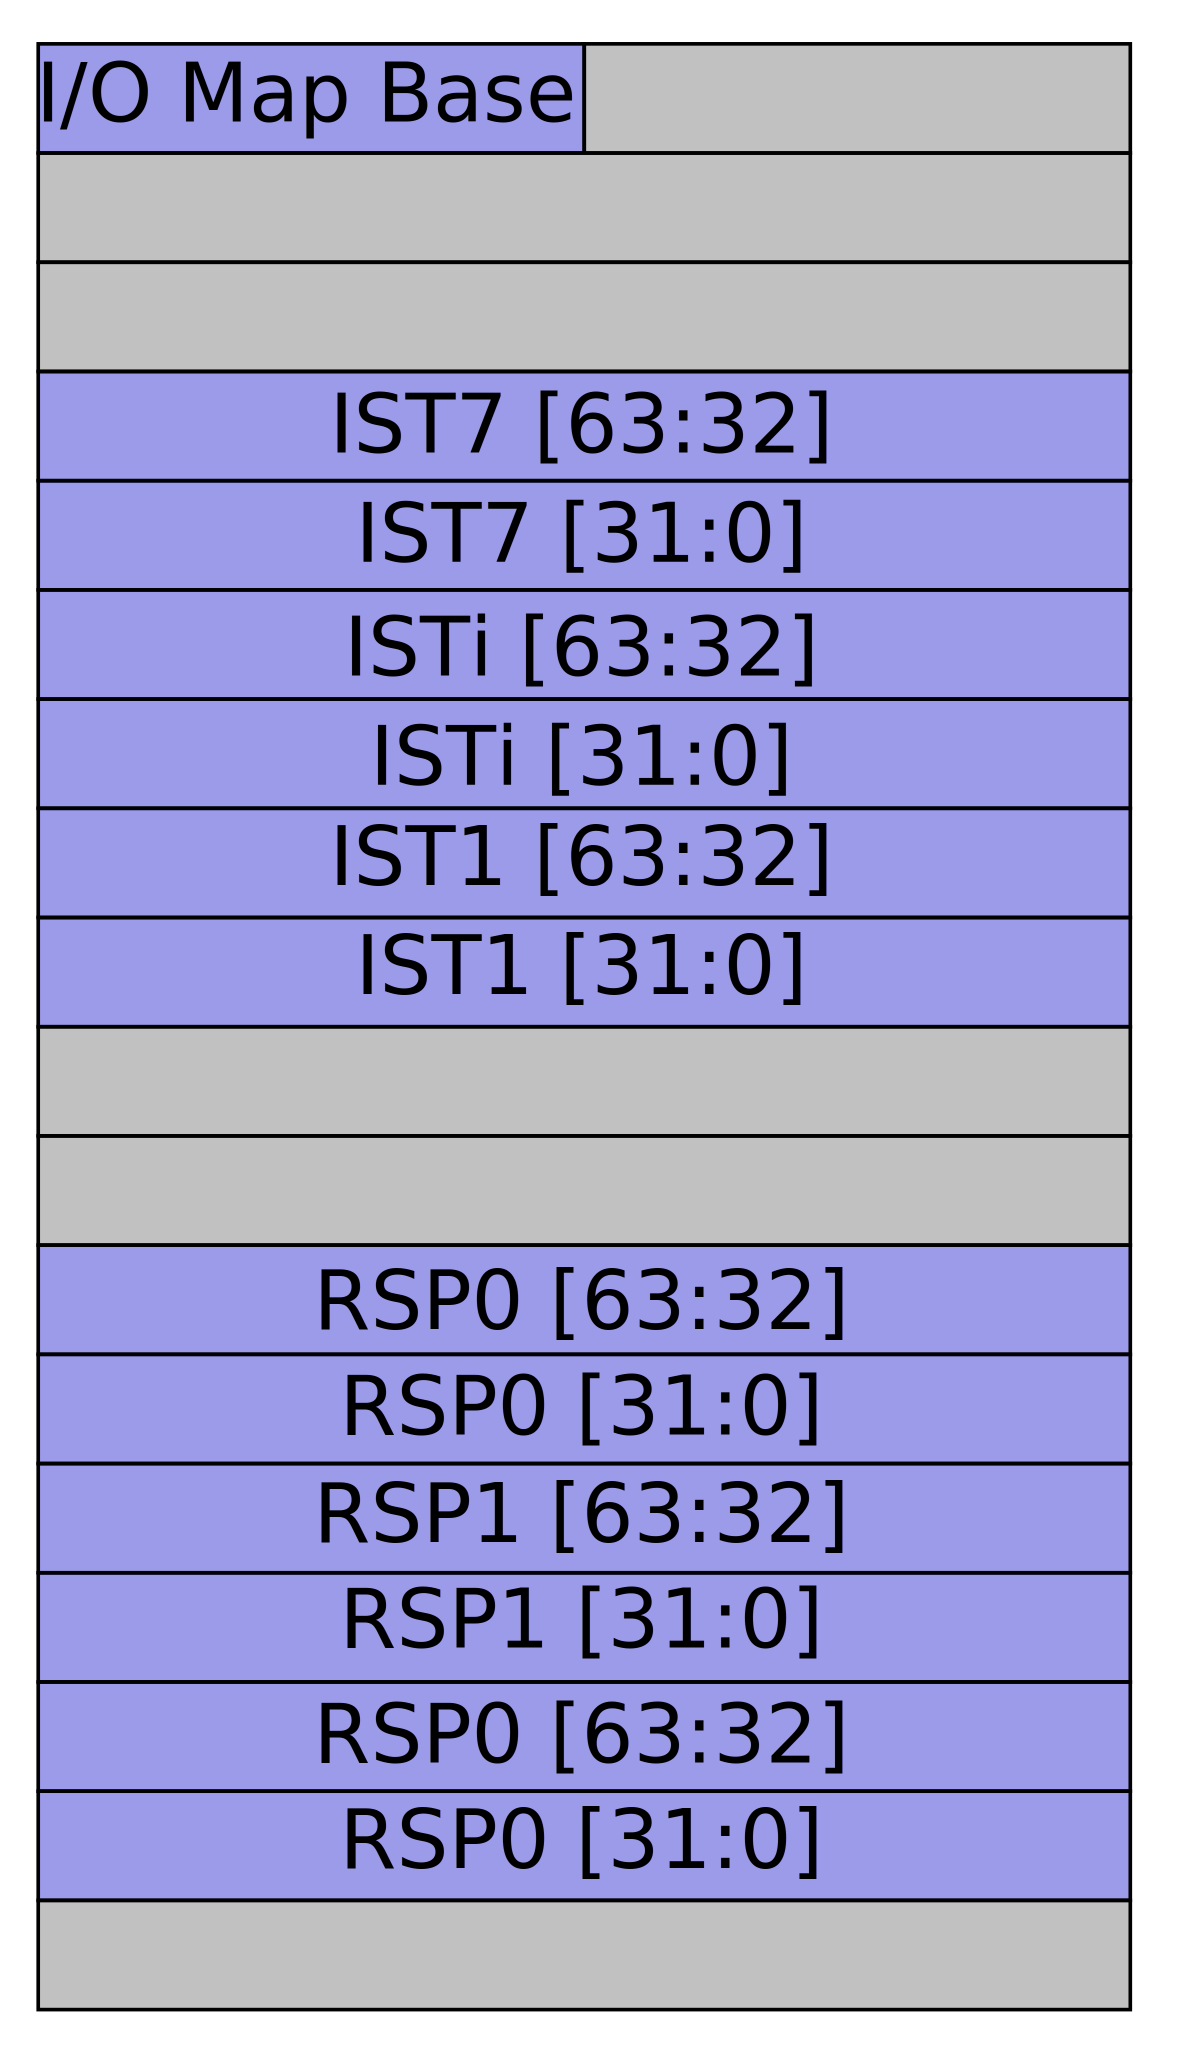
\includegraphics[height=.6\textheight]{tss}
\end{frame}

\begin{frame}
\frametitle{Task State Segment}
\begin{itemize}
    \item<1->"Указание" на TSS хранится в специальном регистре TR
    \begin{itemize}
        \item<2->инструкция LTR записывает значение в TR, а инструкция
             STR читает;
        \item<3->для использования TSS необходимо завести специальный
             дескриптор в GDT
        \begin{itemize}
            \item<3->Base и Limit хранят логический адрес и размер TSS;
        \end{itemize}
        \item<4->селектор дескриптора сохраняется в TR.
    \end{itemize}
\end{itemize}
\end{frame}

\begin{frame}
\frametitle{Task State Segment}
\begin{itemize}
    \item<1->Простой вариант использования TSS:
    \begin{itemize}
        \item<2->создаем по TSS на каждое ядро процессора - один раз, при
             инициализации ядра ОС
        \item<3->при переключении потоков подменяем указатель стека в TSS.
    \end{itemize}
\end{itemize}
\end{frame}

\begin{frame}
\frametitle{Резюме}
\begin{itemize}
    \item<1->Подготовить дескриптор IDT, который будет использоваться для
         системных вызовов.
    \item<2->Создать TSS:
    \begin{itemize}
        \item<3->создать дескриптор, описывающий TSS, в GDT;
        \item<4->загрузить селектор, ссылающийся на дескриптор, в TR.
    \end{itemize}
    \item<5->Не забывать подменять указатель стека в TSS при переключении
         потоков.
\end{itemize}
\end{frame}

\begin{frame}
\frametitle{"Прыжок" в userspace}
\begin{itemize}
    \item<1->Как передать управление в userspace в первый раз?
    \begin{itemize}
        \item<2->инструкция iretq завершает обработчик прерывания и
             передает управление, возможно, понизив уровень привилегий;
        \item<3->инструкция iretq берет свои параметры со стека - подготовим
             стек и вызовем iretq.
    \end{itemize}
\end{itemize}
\end{frame}

\begin{frame}
\frametitle{"Прыжок" в userspace}
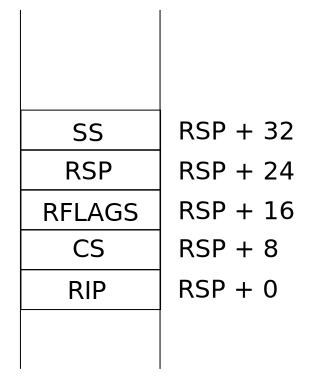
\includegraphics[height=.6\textheight]{intstack}
\end{frame}
